\documentclass[12pt]{beamer}
\usepackage[UTF8]{ctex}
\usetheme{Berkeley}
\usepackage{graphicx}
\usepackage{booktabs}
\usepackage[english]{babel}
\logo{
\includegraphics[height=1cm]{ruc}}
\title[10.47.101.170]{搜索引擎成果展示}
\author{}
\institute[人工智能综合实践2班]
{人工智能综合实践2班 \\ % Your institution for the title page
\medskip
\textit{sherman.hou@gmail.com} % Your email address

}
\date{September 2, 2022}

\begin{document}

\begin{frame}
\titlepage% Print the title page as the first slide
\end{frame}

\begin{frame}{Overview}
\tableofcontents
\end{frame}


%   PRESENTATION SLIDES

\section{搜索算法的优化} %
%------------------------------------------------

\subsection{1. 使用idf对tf加权} %

\begin{frame}{使用idf对tf加权}
\begin{itemize}
\item 1.1 这样加权有什么效果?

使得在计算cosine score时,奖励了包含于的文档个数更少的term,更好地利用这些(文档层面的)低频词的tf来计算score
\item 1.2 负面效果和普适性评估?

一般无负面效果,有理论支持,普适性很强
\end{itemize}
\end{frame}
%------------------------------------------------
\subsection{2. 奖励包含不同关键词更多的网页} %
\begin{frame}{奖励包含不同关键词更多的网页}
\begin{itemize}
\item 2.1 以此应对什么问题?

标准tf-idf模型排序后,很靠前的一些网页实际上包含的关键词“比例”并不高,\alert{其是因为个别词的tf很高才排到前面的} ;
而对于普通用户,在其搜索构词中,关键词数相对少,其对自己输入的各个关键词都抱有的期待,\alert{一般更希望召回含有更多关键词的网页}
\end{itemize}

 
\end{frame}
\begin{frame}{奖励包含不同关键词更多的网页}
\begin{itemize}
\item 2.2 实现方式?

cosine score计算过程里:外层循环遍历query里的关键词,内层循环对包含遍历到的关键词的网页加分(tf * idf);

不难看处,\alert{网页含有多少个关键词就"加了几次分"} ;因此,只要我们在每次加分时再加一个常数数,就实现了对包含更多关键词的奖励
\end{itemize}
\begin{figure}
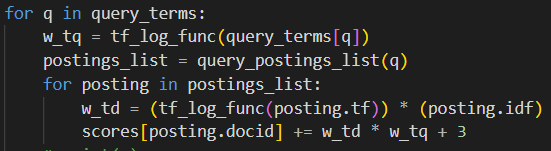
\includegraphics[
width=1\textwidth]{1}
\end{figure}
\end{frame}
\begin{frame}{2.3 负面效果和普适性评估?}
此优化建立在标准cosine score计算模型上,对原本的score进行的调整实际上是\alert{离散}的,含有相等不同关键词的网页获得的加分相同;当我们设置的奖励常数相对(tf * idf)来说很大,完全拉开了含不等数目的不同关键词的网页score间的差距,因此,\alert{本质上实现是一个梯度分类}

这种分类对于”完全取词于同一网页,而没有基于用户需求进行构词“的评测来说肯定是有效的,不会产生负面影响;对于现实中用户自己进行构词的搜索来说,这样的分类弱化了tf的影响,可能会对检索产生负面效果;而参数的存在使得该优化具有更大的普适性,基于检索数据集交叉验证,对奖励参数大小进行调整,可能可以实现理想的效果。
\end{frame}

\subsection{3. 奖励长度更长的网页} %
\begin{frame}{奖励长度更长的网页}
\begin{itemize}
\item 3.1 原因与实现方式?

尝试不对cosine score模型中的文档向量作归一化...评测得分“居然”上升了许多,猜测是因为后勤集团域名下的网页的长短两极分化严重,而评测样例中最优网页大多为长网页
\item 3.2  普适性评估?

普适性无疑是差的,只是基于后勤集团域名下的网页特点和评测样例特点;且与cosine score相关理论相违背
\end{itemize}
\end{frame}

\subsection{4. 奖励包含完整query的网页} %
\begin{frame}{奖励包含完整query的网页}
\begin{itemize}
\item 4.1  以此应对什么问题?

通过上述优化,我们奖励了包含关键词更多的网页,\alert{但实际上我们没有规定这种包含是连续还是间断},倘若实现\alert{对”是否连续地包含所有关键词“的判断},我们的排序模型会更加稳健。
\end{itemize}
\end{frame}
\begin{frame}{4.2 如何实现?}
\begin{itemize}
\item 保存位置索引

回顾一下我们实现tf-idf模型构造的倒排索引,可看作一个字典,key是词,value是“文档”构成的列表,这里的文档作为列表的元素,\alert{只包含docid序号是不够的},因此我们不妨构造一个新的数据类型(对应于课堂ppt中提到的\textbf{class Posting}),其中打包保存了\alert{docid,tf,以及idf};

\alert{而如若考虑”是否‘连续地‘包含关键词“,只保存这些参数是不够的},我们还需要一个由”文档内的位置索引“构成的列表。我们可以将切词后保存(词,docid)对的过程改进为保存\alert{(词,docid,位置索引)},而在后续构造倒排索引时\alert{将同一docid对应的位置索引构成一个列表,也存放到Posting中。}

\end{itemize}
\end{frame}
\begin{frame}{4.2 如何实现?}
\begin{itemize}
\item 遍历与递归判断

\end{itemize}
\begin{figure}
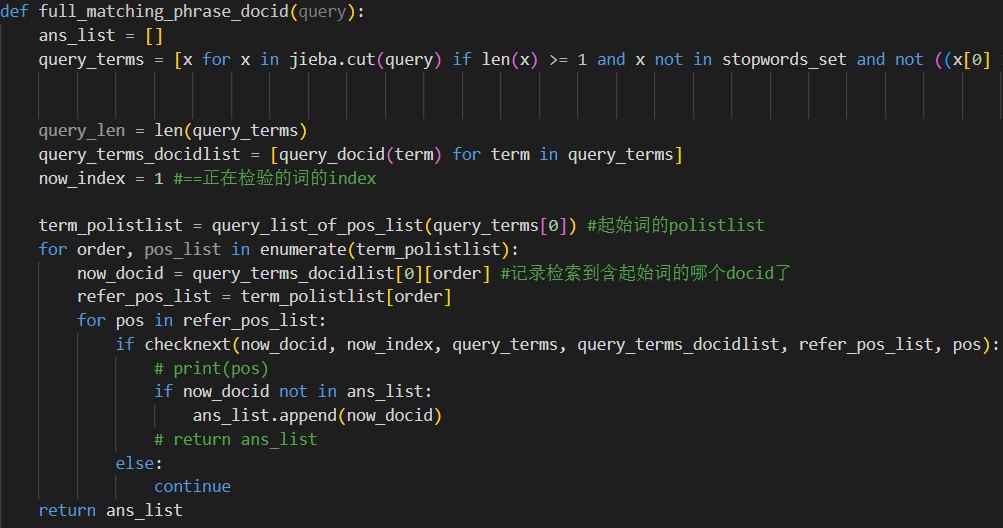
\includegraphics[
width=1\textwidth]{9}
\end{figure}

\end{frame}
\begin{frame}{4.2 如何实现?}
\begin{itemize}
\item 遍历与递归判断

\end{itemize}
\begin{figure}
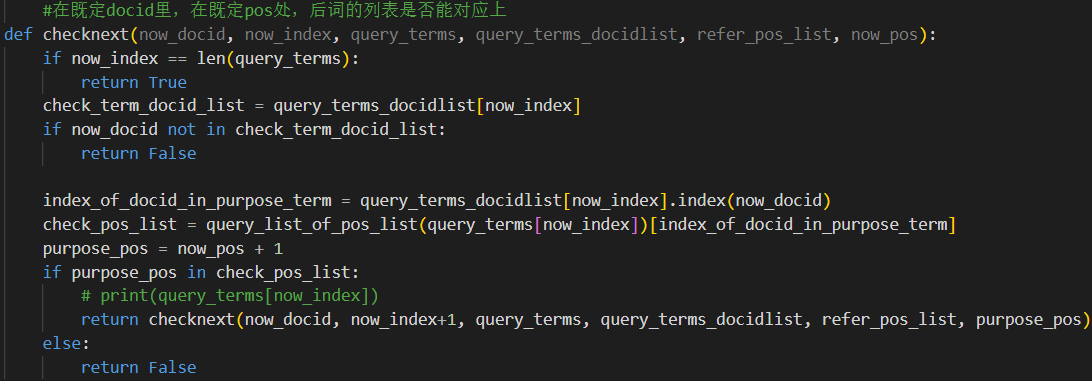
\includegraphics[
width=1\textwidth]{2}
\end{figure}
\begin{itemize}
\item 对cosine score模型计算出的分数加权:

与前面所说的第二种优化类似,这一优化本质上也是分类,我们对列表内docid的score放大相同的倍数,将倍增调整后的score重新排序,作为最终的score
\end{itemize}
\end{frame}
\begin{frame}{4.3 效果和普适性评估?}
此优化中,我们检验的是是否返回完整的query,为一个\alert{二分类};没有改变同类网页之间的cosine score排序,通过对cosine score的调整来”标记分类“,相对于再另外设置bool变量来说是一种更简单的实现方式。

该优化直接了实现”必须包含某短语“需求的搜索;在此基础上,通过对用户的细化输入的获取,我们可以实现一些高级搜索

是否需要实现对含有的query的子串的最长长度的标记呢? 我觉得\textbf{由于query本身的长度差异,连续性文本出现的价值也有差异;例如用户的query为一个单词加一个较短短语,对网页中此较短短语完整包含的奖励会冲击另一个同样重要的单词带来的影响。}
或许我们可以尝试当且仅当query较长,且匹配子串占比较大的时候才进行奖励
\end{frame}
%------------------------------------------------
\section{Web UI网页优化}

\subsection{1. 美观性} %
\begin{frame}{Web UI网页的美观性}
\begin{itemize}
\item 背景图片,小图标,字体字号调整
\item 鼠标悬浮时的效果
\item 访问过的网页色彩变动
\item 透明度、标题突出
\item 对网页呈现对不同浏览器,不同设备的适应性
\item 返回页面中当前搜索词呈现方式与位置
\end{itemize}
\end{frame}

\subsection{2. 摘要选择与关键词标红显示} %
\begin{frame}{摘要选择与关键词标红显示}
\begin{figure}
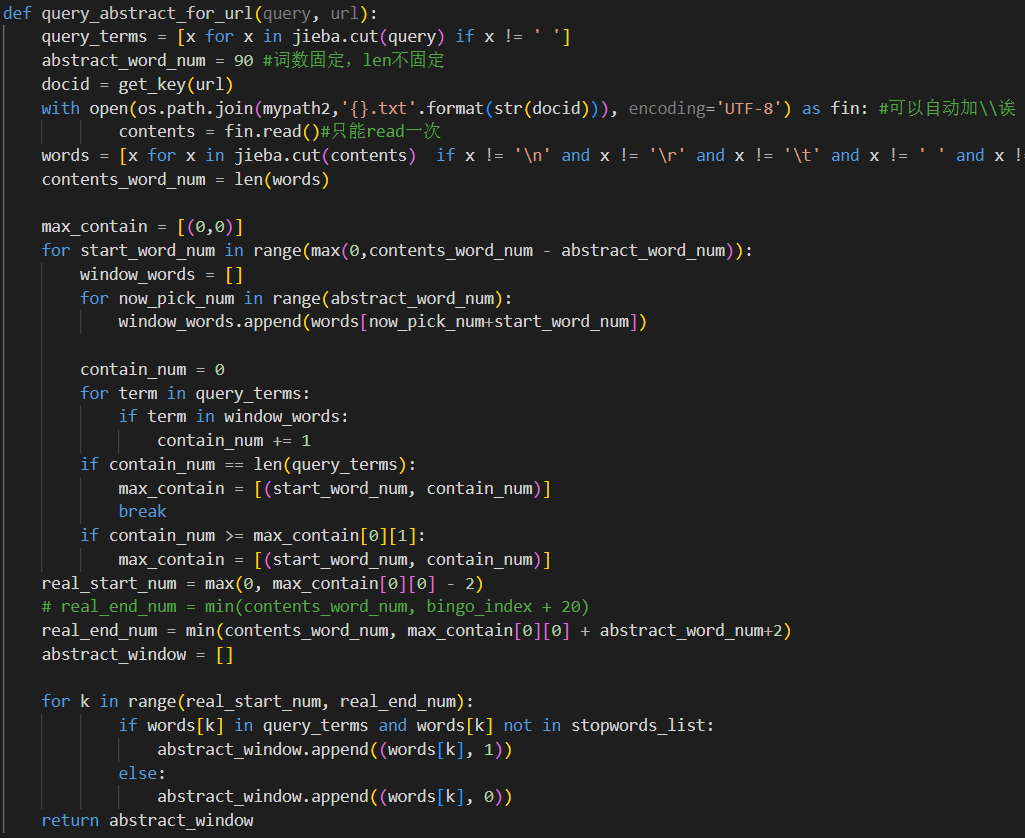
\includegraphics[
width=0.9\textwidth]{6}
\end{figure}
\end{frame}
\begin{frame}{摘要选择与关键词标红}
\begin{figure}
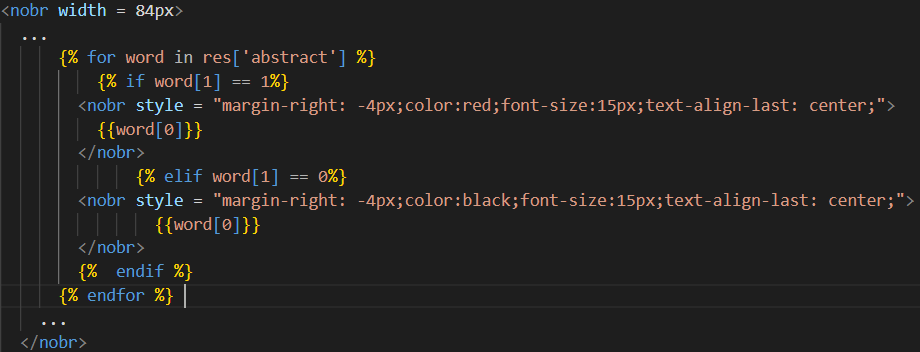
\includegraphics[
width=1\textwidth]{7}
\end{figure}

\end{frame}

\subsection{3. 标题内容优化与去重} %
\begin{frame}{标题内容优化与去重}
\begin{figure}
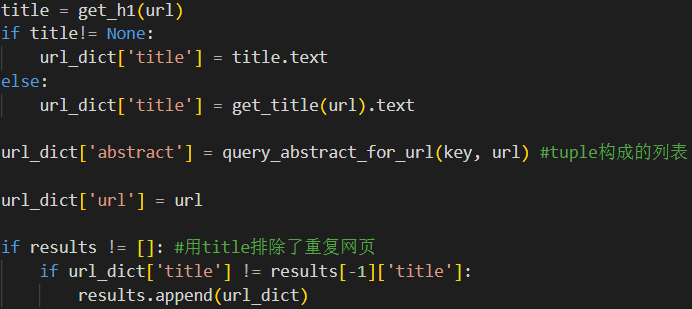
\includegraphics[
width=0.9\textwidth]{3}
\end{figure}
\end{frame}
\subsection{4. 对特殊搜索的适应性} %
\begin{frame}{对特殊搜索的适应性}
\begin{itemize}
\item 空字符串
\item 无效检索词
\item 过长检索词
\item 未找到任何含有关键词的网页
\begin{figure}
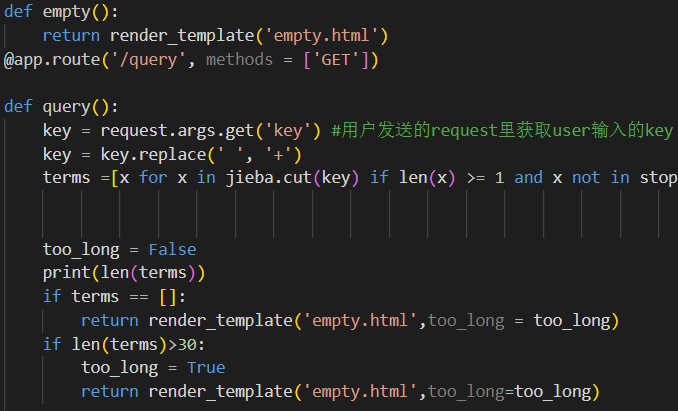
\includegraphics[
width=0.6\textwidth]{4}
\end{figure}
\begin{figure}
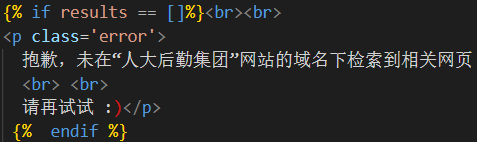
\includegraphics[
width=0.6\textwidth]{8}
\end{figure}
\end{itemize}
\end{frame}
%----------------------------------------------------------------------------------------

\end{document} 